\chapter{Choosing the Field Before Building the Company}

This chapter comes from a short School of Hard Knocks entrepreneurship interview segment, curated by LazyingArt LLC through Video2Book. The speaker is asked why solar sales stood out as a place to build. His answer is not a finished theory of renewable energy. It is a compact decision story: begin with a long-horizon industry scan, bracket personal opinion, admit what we do not yet know, get close enough to learn, and only then decide whether to build.

\section{The Opening Question: Why Solar Sales?}

The interviewer begins with the practical question. What was it about solar sales that made the speaker think, in effect, that a company could be built there? The answer matters because it separates an entrepreneurial origin story from a slogan. The speaker does not begin by saying that he already understood solar, energy policy, or sales organizations. He begins earlier, with the period when he was still trying to decide which fields were worth entering.

He places the search during his brief time in college:

\begin{equation}
t_0 \approx 2014\text{--}2016.
\end{equation}

That date is not used as a precise quantitative datum. It is the setting of the decision. At time \(t_0\), the problem was not yet, ``How do I build a solar sales company?'' The problem was more basic: among all possible industries, where should we spend our attention, learning energy, and early career risk?

\section{The Twenty-Year Industry Test}

The speaker's filter was a long-horizon growth question. He says that he was looking at emerging industries and asking what would be bigger in the next twenty years than it was at the time. Written as a compact decision rule, the test is:

\begin{equation}
\text{Industry scale}_i(t_0+20) >
\text{Industry scale}_i(t_0).
\end{equation}

This is not a valuation formula. It is a discipline for attention. Before asking whether we like an industry, understand it, or know how to operate inside it, we first ask whether the field itself is likely to expand.

The important feature of the rule is its directionality. The speaker is not claiming to know exact market size, adoption curves, or profit margins. He is using the expected direction of an industry as a first screen. In entrepreneurship, that first screen matters because a growing field can forgive some early ignorance. A shrinking field often punishes even competent effort.

\subsection{Question \& Answer}

\paragraph{Question.}
How do we evaluate an industry when people have strong feelings about it, or when political opinions make the topic noisy?

\paragraph{Answer.}
The speaker's move is to bracket opinion long enough to ask a colder question: what is going to be bigger twenty years from now than it is today? Personal fit still matters, but it comes later. The first pass is not, ``Do I already agree with the industry?'' or ``Do I already understand it?'' The first pass is:

\begin{equation}
G_i =
\begin{cases}
1, & \text{if the field appears likely to grow over the horizon},\\
0, & \text{otherwise}.
\end{cases}
\end{equation}

This binary notation is only an editorial shorthand for the transcript's reasoning. The speaker does not present a formal model. But the shorthand preserves the rhythm of the answer: separate trend direction from personal preference, then decide whether the field deserves study.

\section{The Candidate Set}

After establishing the growth filter, the speaker names examples that were visible to him: technology, artificial intelligence, robotics, renewable energy, and crypto. We can record the set as:

\begin{equation}
\mathcal{C}
=
\{\text{tech},\ \text{AI},\ \text{robotics},\ \text{renewable energy},\ \text{crypto}\}.
\end{equation}

The list should be read modestly. It is not a ranked portfolio, not a prediction table, and not a claim that every listed field has the same risk. The point is that solar sales entered his attention through the broader category of renewable energy, which sat among several fields he thought could become larger over time.

The chapter should preserve that order of discovery. Solar is not introduced as a field he had already mastered. It is introduced as one possible doorway inside a larger search for expanding industries.

\section{The Knowledge Gap As An Entry Problem}

The next turn is crucial. The speaker says he did not know much about any of those industries. That admission prevents the story from becoming a false tale of early expertise. The mechanism is not omniscience. The mechanism is study plus proximity.

We can write the learning process as an update rule:

\begin{align}
K_{n+1} &= K_n
+ \Delta K_{\text{study}}
+ \Delta K_{\text{access}},\\
F_{n+1} &= F_n
+ \Delta F_{\text{exposure}}.
\end{align}

Here \(K_n\) represents working knowledge after \(n\) steps, and \(F_n\) represents tested fit. This is not a transcript equation; it is a clean way to express the speaker's sequence. Study increases knowledge from the outside. A foot in the door increases knowledge from the inside. Exposure tests whether the industry is a good fit.

The spoken order is important:

\begin{enumerate}
\item Find a field that looks likely to grow.
\item Study it enough to become less blind.
\item Get a foot in the door.
\item Learn whether the field fits.
\item Build around it only after that evidence begins to accumulate.
\end{enumerate}

This order is more conservative than the usual myth of the founder who simply sees the future. The speaker is describing staged commitment.

\section{A Narrow Process Diagram}

Because no validated visual frame contains useful board content, the only appropriate figure here is a transcript-derived reconstruction. It should be read as a process diagram, not as something drawn in the source video.

\begin{figure}
\centering
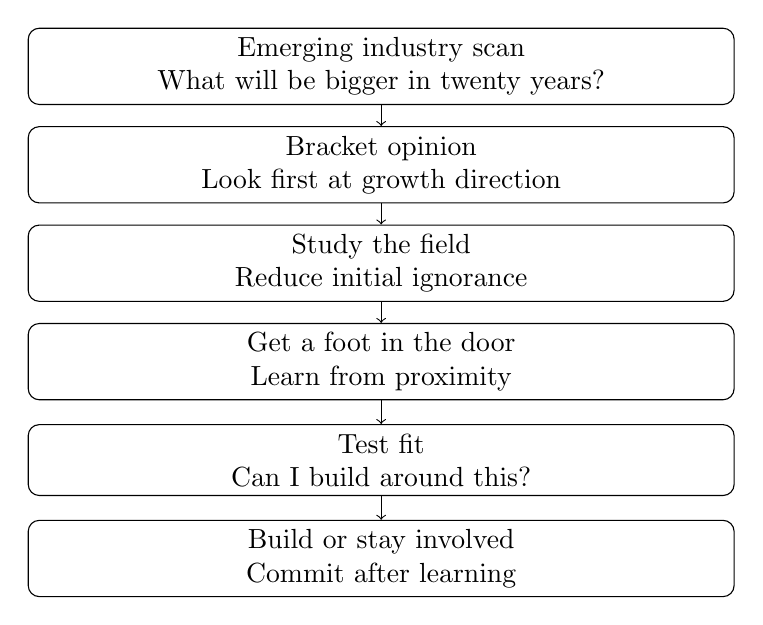
\begin{tikzpicture}[
  node distance=1.25cm,
  box/.style={
    draw,
    rounded corners,
    align=center,
    text width=0.72\linewidth,
    minimum height=0.85cm
  }
]
\node[box] (scan) {Emerging industry scan\\What will be bigger in twenty years?};
\node[box, below of=scan] (filter) {Bracket opinion\\Look first at growth direction};
\node[box, below of=filter] (study) {Study the field\\Reduce initial ignorance};
\node[box, below of=study] (entry) {Get a foot in the door\\Learn from proximity};
\node[box, below of=entry] (fit) {Test fit\\Can I build around this?};
\node[box, below of=fit] (build) {Build or stay involved\\Commit after learning};

\draw[->] (scan) -- (filter);
\draw[->] (filter) -- (study);
\draw[->] (study) -- (entry);
\draw[->] (entry) -- (fit);
\draw[->] (fit) -- (build);
\end{tikzpicture}
\caption{A transcript-derived reconstruction of the speaker's entry logic: scan for growth, learn, gain access, test fit, then build or participate.}
\end{figure}

This figure keeps the structure narrow for pocket-size export. It also keeps the evidentiary boundary clear: the process is reconstructed from the transcript, not from a blackboard or slide.

\section{A Worked Example: Renewable Energy As The Doorway}

Now let \(i=\text{renewable energy}\). The speaker's logic does not require him to begin with complete expertise in renewable energy. It requires only that renewable energy pass the first directional screen:

\begin{equation}
\text{Industry scale}_{\text{renewable energy}}(t_0+20)
>
\text{Industry scale}_{\text{renewable energy}}(t_0).
\end{equation}

Once the field passes that screen, the next question is not yet, ``What company should I start?'' It is:

\begin{equation}
\text{Can I obtain access that increases } K
\text{ and tests } F?
\end{equation}

In ordinary language, can we get close enough to learn the business and see whether we fit the work? Solar sales becomes plausible because sales can be an entry path into the renewable-energy field. It is a way to touch customers, incentives, objections, operations, and demand without pretending to understand the entire industry on day one.

A compact editorial model for the opportunity is:

\begin{equation}
\text{Opportunity}_i
\approx
\text{growth direction}_i
+
\text{access}_i
+
\text{learnability}_i
+
\text{fit}_i.
\end{equation}

The approximation sign is deliberate. This is not arithmetic. It is a reminder that the speaker's reasoning has several parts. Growth alone is not enough. Access alone is not enough. Fit alone is not enough. The entrepreneurial opportunity begins to appear when these pieces point in the same direction.

\section{From Involvement To Building}

The final beat broadens the lesson. The speaker says it did not have to be starting a business. It only had to be involvement in those industries. That line is easy to pass over, but it changes the structure of the decision.

Starting a company is not the first variable. The first variable is industry exposure. We can write the staged commitment as:

\begin{align}
\text{Stage 1} &: \text{enter a growing field},\\
\text{Stage 2} &: \text{learn from study and proximity},\\
\text{Stage 3} &: \text{test personal and commercial fit},\\
\text{Stage 4} &: \text{build, operate, or remain strategically involved}.
\end{align}

This is the mature part of the answer. The speaker is not saying, ``I saw solar, therefore I immediately knew the company.'' He is saying, ``I looked for expanding fields, found a path to get close, and treated involvement as the first commitment.'' Building comes after enough contact with reality.

\section{Summary}

The chapter's spine is a simple but useful entrepreneurial sequence. During the 2014--2016 period, the speaker looked for industries likely to be larger twenty years later. He separated that growth question from personal or political preference, named several candidate sectors, admitted limited knowledge, and treated study plus access as the way to learn. Solar sales mattered because it offered a doorway into renewable energy, not because the full company was obvious from the beginning.

The lesson is staged commitment: choose the field before choosing the company, get close enough to learn, test fit before overcommitting, and build only when growth, access, learnability, and fit begin to reinforce one another.